\documentclass[a4paper,12pt]{report}
\usepackage{color}
\usepackage{hyperref}
\hypersetup{
    colorlinks,
    citecolor=black,
    filecolor=black,
    linkcolor=black,
    urlcolor=black
}
\setcounter{secnumdepth}{0}
\usepackage{graphicx}
\usepackage{epstopdf}
\usepackage{amsmath}
\usepackage[table,xcdraw]{xcolor}
\usepackage{amssymb}
\usepackage{listings}
\definecolor{anti-flashwhite}{rgb}{0.95, 0.95, 0.96}
\lstset{ 
  backgroundcolor=\color{anti-flashwhite}
  }
\begin{document}
\title{
\textbf{Operating Systems - II: CS3523}\\~\\
\begin{large}
\textbf{Implementing TAS, CAS \& Bounded Waiting CAS\\
Mutual Exclusion Algorithms\\}
\end{large}
\begin{large}
\textbf{Assignment Report}
\end{large}
}
\author{\textbf{Sagar Jain - CS17BTECH11034}\\}
\maketitle
\begin{large}
\tableofcontents
\end{large}
\newpage
\section{Salient Features of Program Design}
To implement TAS \& CAS, we need their operation to be atomic. In plain CPP we can atmost guarantee the atomic update of a single variable(a single instruction), however we cannot be sure about interleaving of instructions while using a  manual implementation of test\_and\_set(using \textit{mutex} would beat the purpose of the assignment). This is the reason why I have chosen to use the funcitons from \textit{\textbf{atomic}} header \textit{\textbf{test\_and\_set}, \textbf{compare\_exchange\_weak}}\\
The following are the key points involved in designing each of the three programs.
\begin{enumerate}
\item For TAS, as mentioned, I have made use of :\\ \textbf{\textit{locker.test\_and\_set(memory\_order\_acquire)}} to enter the critical section and \textbf{\textit{locker.clear(memory\_order\_release)}} to exit the critical section. Here locker is of type \textbf{\textit{atomic\_flag}} which can be updated/read atomically by the aforementioned functions.
\item For CAS, as mentioned, I have made use of: \\ \textbf{\textit{locker.compare\_exchange\_weak(expected,1)}} to enter the critical section and \textbf{\textit{locker.operator=(0)}} to exit the critical section. Here locker is of type \textbf{\textit{atomic\_int}} which can be updated atomically by the aforementioned functions, \textbf{\textit{expected}} is a varibale with value 0.
\item For bounded CAS, the implementation is as follows:
\begin{enumerate}
\item There is a global array \textbf{\textit{waiting}} to store the waiting status of every thread.
\item The variable \textbf{\textit{key}} is updated by calls to compare and exchange.
\item To exit the critical section the running thread then looks for the next waiting thread and sets it value in waiting array to false. This is the thread that runs next.
\end{enumerate}
\item To measure the waiting times, I have used a global waiting matrix which is updated whenever a thread enters the critical section.
\item For time measurements I have used \textbf{\textit{chronos}}.
\item For writing to files I have used \textbf{\textit{fprintf}} as it does not have concurrency issues.
\end{enumerate}
\newpage
\section{Program Output}
The output from the any of the three programs gives a log of the events that take place, namely, the request to enter critical section by a thread, the entry of a thread into its critical section, the exit of thread from its critical section. To prove mutual exclusion is ensured one can check the logs and it is observed that after the entry of one of the threads into the critcal section, no other thread enters its respective critcal section before the exit of the thread that is already in its critical section.
\textbf{fprintf }has been used since not all logging statements are in the critical section, so there can be an interleaving of the print statements, leading to meaning less logging. fprinf does not have the concurrency issue.
\newpage
\section{Results \& Graphs}
We have three graphs which have been made by running the three solutions for mutual exclusion with varying number of proceses.The graphs have been generated using \url{https://github.com/Sagox/IIT-Hyderabad-Courses/blob/master/OS_II_Assignments/Assignment_2/collect_output.py}, in this file we average every reading five times. Each of the following graphs gives insight into an aspect of the solutions.\\\\
\begin{center}
\begin{large}
\textbf{Average Waiting Time vs Number of Threads}
\end{large}
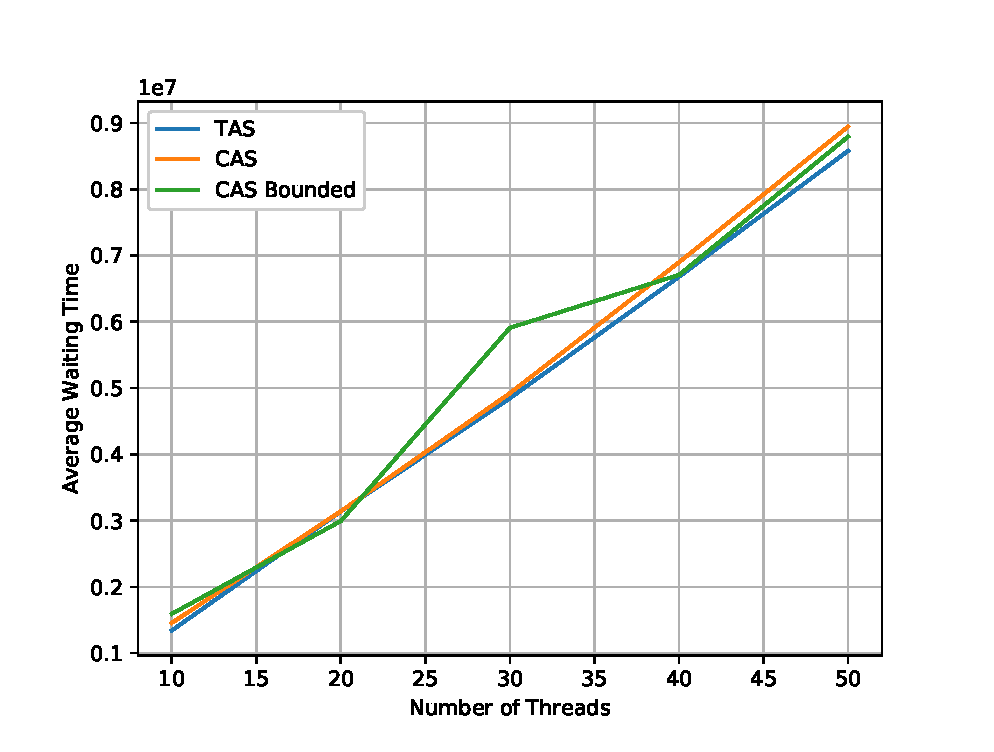
\includegraphics{avg.eps}
\end{center}
\begin{center}
\begin{large}
\textbf{Maximum Waiting Time vs Number of Threads}
\end{large}
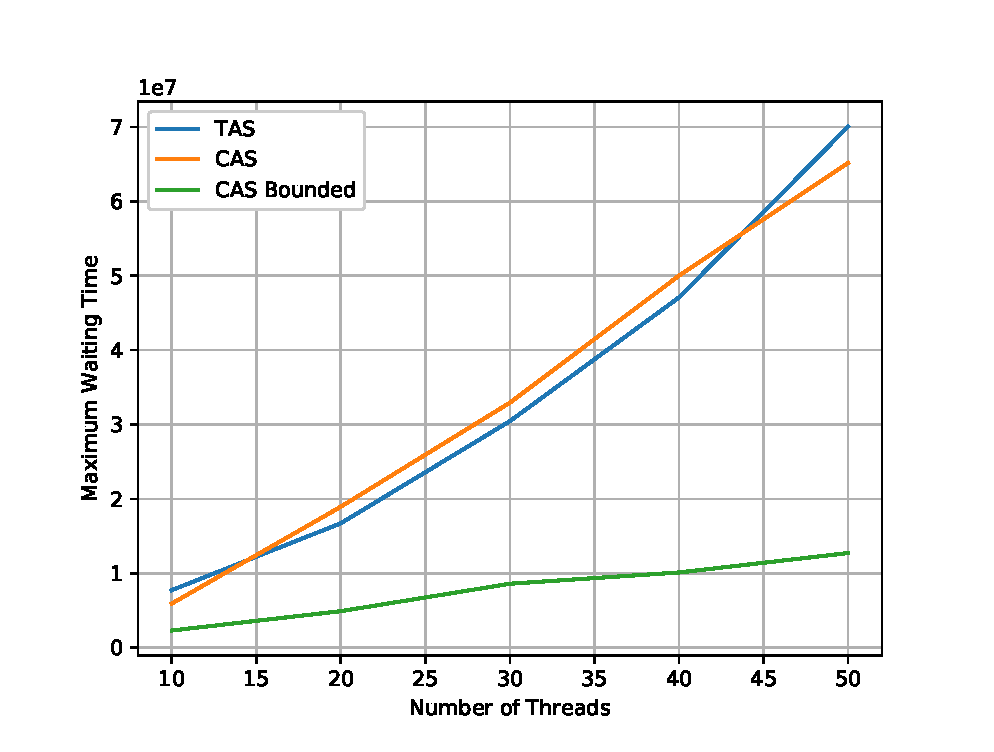
\includegraphics{max.eps}
\end{center}
\newpage
\begin{center}
\begin{large}
\textbf{Standard Deviation of Waiting Time vs Number of Threads}
\end{large}
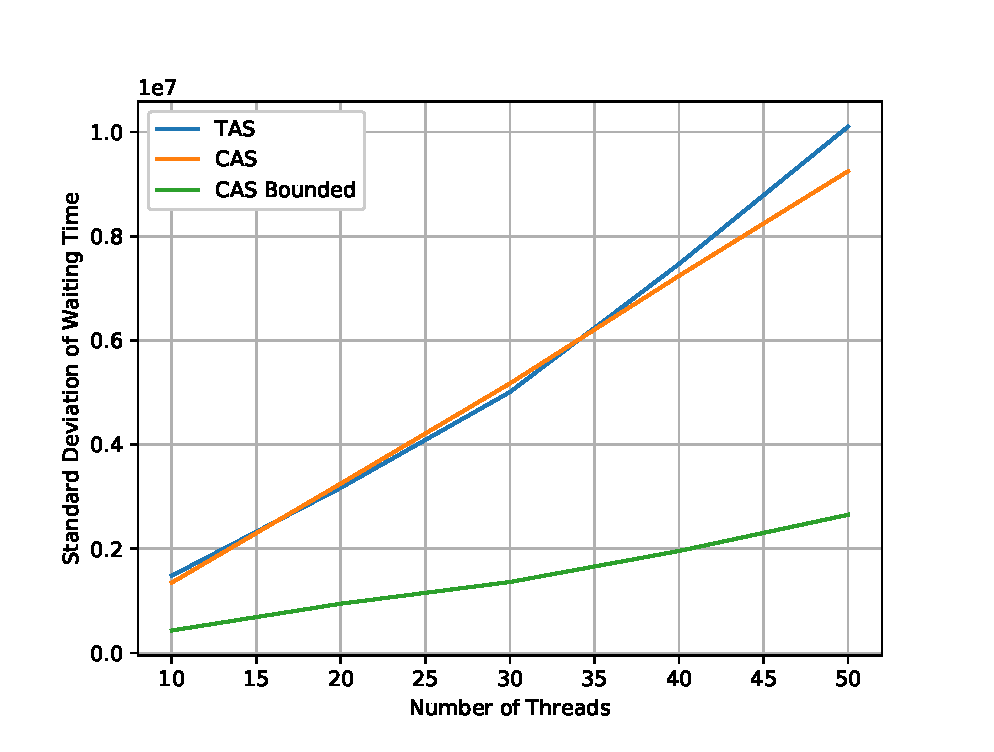
\includegraphics{sd.eps}
\end{center}
\newpage
\section{Explaination of Results}
The following is the interpretation of each of the graphs presented above:
\begin{enumerate}
\item The average waiting time of threads gives th following insights:
\begin{enumerate}
\item The average waiting time increases for all the three with increase in the number of threads, this is obvious since each thread would end up waiting for more number of threads.
\item The average waiting times for all of the three solutions is similar, albeit slightly higher for CAS and Bounded CAS, this can be attributed to the fact that they involve more instructions when compared to TAS.
\end{enumerate}
\item The maximum waiting time is also not surprising.
\begin{enumerate}
\item The maximum waiting time increases with the number of threads since now every thread waits for more number of other threads to exit their critical section. This is observed in all the three solutions.
\item The maximum waiting time for CAS Bounded is much less compared to TAS and ordinary CAS, this is expected since we explicitly try to avoid starvation in bounded CAS.
\end{enumerate}
\item The standard deviation of waiting time also is as expected, since we have avoided starvation in Bounded CAS, the values for waiting time do not shoot up for any thread and this keeps the variance down, but the other two do not have this provision, which results in some threads having very large waiting times, this leads to a big value of variance.
\end{enumerate}
\end{document}